\documentclass[12pt,a4paper]{article}

\usepackage{url}
\usepackage{appendix}
\usepackage[british]{babel}
\usepackage{amsmath}
\usepackage{hyperref}
\usepackage{graphicx}
\numberwithin{equation}{section}
\numberwithin{figure}{section}
\numberwithin{table}{section}

\usepackage[round]{natbib}
\bibliographystyle{natbib}
\def\bibsection{\section*{References}}

% Wrap around which gives all figures included the [H] command, or places it "here". This can be tedious to code in Rmarkdown.
\usepackage{float}
\let\origfigure\figure
\let\endorigfigure\endfigure
\renewenvironment{figure}[1][2] {
    \expandafter\origfigure\expandafter[H]
} {
    \endorigfigure
}

\let\origtable\table
\let\endorigtable\endtable
\renewenvironment{table}[1][2] {
    \expandafter\origtable\expandafter[H]
} {
    \endorigtable
}

\def\tightlist{}

\bibpunct[:]{(}{)}{;}{a}{,}{,}

\renewcommand{\baselinestretch}{1.5}

\begin{document}

\begin{titlepage}

\begin{center}
{\Huge \bf Comparing Facebook's Prophet Forecasting to an ARIMA Model: A
Diebold-Mariano Evaluation of the Top40 Index}\\
\today\\
Marvelous Mubenesha ( MBNMAR005)\\
{\tt MBNMAR005@uct.co.za}
\end{center}

\begin{abstract}
Facebook's data science team open-sourced Prophet, a package that allows
analysts to forecast a wide range of business time series at-scale.
Prophet employs intensive Bayesian modelling in two tiers. Purely
through MAP parameter estimation, and in a quasi-Bayesian form through
an automated forecast evaluation that enables analyst to improve the
model if it falls short when compared to other models. This paper assess
the predictive accuracy of Prophets' forecasts to those of an ARIMA
model that was identified using the Box-Jenkins methodology. This is
achieved through a Diebold-Mariano evaluation of the rolling period
forecast errors of returns on the FTSE/JSE Top40 Index across daily,
weekly and monthly time horizons. The results of the study suggest that
there is insufficient evidence to conclude that the forecasting models
have unequal predictive ability within the scope of the JSE/Top40 Index.
\noindent
Keywords: prophet forecasting, arima forecasting, Box-Jenkins methodology,Diebold-Mariano test,multi-step rolling window forecasts, FTSE/JSE Top40 index.
\end{abstract}
\end{titlepage}

\pagenumbering{arabic}

\section{\texorpdfstring{Introduction\label{Introduction}}{Introduction}}\label{introduction}

In business, including that involving the stock market, analysts require
a large number of time series forecasts to inform decision making. The
challenge with existing reliable approaches to forecasting time series
data are that the models require a considerable background in statistics
to build and adapt to prevailing market conditions when needed. Several
authors have recommended automatic forecasting, which refers to
algorithms that can automatically forecast a large number of univariate
time series. However, the forecasts generated by these methods have been
found to be brittle as well as inflexible in allowing for prior
information to be incorporated into the forecasting model (Taylor and
Letham 2017). In February of 2017, Facebook's Core Datascience team open
sourced ,Prophet, their time series forecasting tool whose main selling
point is that it enables ``forecasting-at-scale''. A term coined by the
data science team which is defined as, ``an approach that allows a large
number of analysts to forecast a large number and variety of business
time series'' (Taylor and Letham 2017). It has the added advantage of
being less `expensive' than other alternatives. In addition, it is
specifically prefarable over ARIMA models because of its non-linearity,
flexibility and ability to accomodate varying time intervals (Taylor and
Letham 2017).

The objective of this paper is to compare the rolling period forecasts
generated by Prophet (which uses automated, intensive Bayesian Modelling
to `forecast-at-scale'), to those obtained by an ARIMA model
(constructed through the Box-Jenkins methodology), through a
Diebold-Mariano evaluation of the JSE Top40 Index. The study is
particularly useful because analysts from a wide background can
automatically forecast stock price returns, and incorporate their prior
knowledge in the model , without a wholesome understanding of the
statistical intricacies involved.

The paper is organized as follows. A review of literature relating to
stock price forecasting with ARIMA models and other alternative
approaches is introduced to give the reader background information on
research relating to the subject matter. Thereafter, theory relating to
the mathematical formulation and estimation of both the ARIMA and
Prophet models is included in sections 2.2 and 2.3 respectively, to
build the readers understanding of what the models look like and how
they operate. Information relating to the data that was used in this
study is contained in section 3, after which, the methodology used to
answer the research question is described in section 4. Section 5,
contains the results obtained when the methodology was executed, whilst
section 6 includes a discussion of the results and how they can be
interpreted to answer the research question. Lastly, the conclusion in
section 7 highlights the main findings of the study and recommends
further areas of research.

\section{Background}\label{background}

In this section we will briefly review literature that relates to the
comparison of different approaches to forecasting stock returns. This
will include both traditional approaches as well new methods such as
automatic forecasting, machine learning techniques and quasi-Bayesian
forms which incorporate analysts' prior information. The review of
literature is concluded with a brief introduction to the Diebold-Mariano
evaluation and an outline of its suitability for the purpose of this
study. The theoretical and mathematical formulation of an ARIMA
forecasting model is then briefly introduced. Thereafter, the
theoretical framework and mathematical formulation of Facebooks' Prophet
forecasting tool is discussed. Specific attention is drawn to Prophets
distinguising features to give the reader an understanding of the value
that this forecasting technique can potentially add to stock price
prediction. Lastly, the Diebold-Mariano Evaluation technique is
introduced as a method of formally testing superior predictive accuracy
between two forecasting models.

\subsection{Literature}\label{literature}

\subsubsection{Forecasting stock prices using the ARIMA
model}\label{forecasting-stock-prices-using-the-arima-model}

ARIMA models have been widely used as a standard model to forecast
financial data and have been shown to yield acceptable forecasting
errors (Adebiyi, Adewumi, and Ayo 2014). Adebiyi, Adewumi, and Ayo
(2014) used the Box-Jenkins methodology to build short-term stock price
prediction models for stocks on the New York Stock Exchange(NYSE) and
the Nigerian Stock Exchange(NSE). Their results showed that the
prediction errors of the model were within acceptable bounds.

ARIMA models rely on the assumption that residuals are
heteroskedastic(they have a constant variance) and normally distributed,
however, some financial data displays heteroskedasticity making GARCH
models more applicable. This theory is backed by a study conducted by
Mutendadzamera and Mutasa (2014) who compared the ability of ARIMA and
GARCH models to forecast stock prices on the Zimbabwean Stock Exchange
(ZSE). They found that the GARCH model outperforms the ARIMA model which
suggests that the residuals are heteroskedastic. This is a case in point
for emerging market stocks. The researchers noted that poor liquidity in
the market could be a cause of the results they observed (Mutendadzamera
and Mutasa 2014).

\subsubsection{Forecasting stock prices using alternative methods: The
case of Artificial Neural Networks and Hybrid
Models}\label{forecasting-stock-prices-using-alternative-methods-the-case-of-artificial-neural-networks-and-hybrid-models}

Though the ARIMA model is tractable given that it is simple,
interpretable and yields forecasts that are significantly accurate when
compared to other methods, it has its limitations. The most popular
being its inability to capture non-linear patterns in data, even after
its evolution from the standard form to more adaptable formulations
(Moreno, Pol, and Gracia 2011). Over the past two to three decades with
the evolution of computational power and statistical advancement, other
stock price prediction methods have been proposed, the most prominent
being a machine learning approach called Artificial Neural
Networks(ANNs)(Lin, Yang, and Song 2009). Also popular amongst the new
stock price forecasting approaches are hybrids of existing methods that
incorporate the benefits of different approaches.

Artificial Neural Networks (ANNs) are a multi-layered perceptron as
illustrated in figure 1.\\
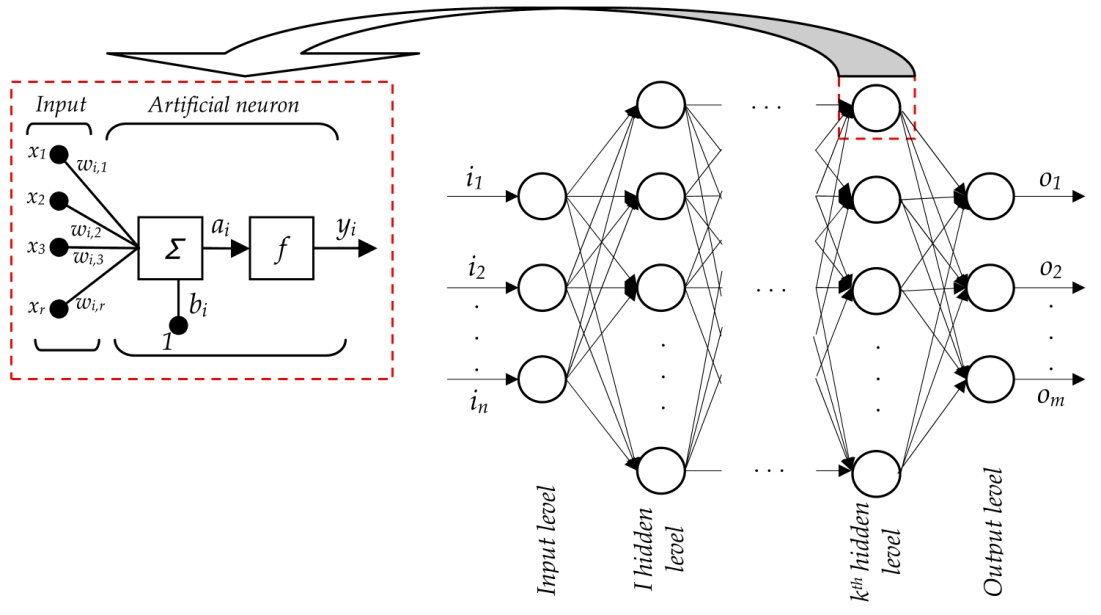
\includegraphics{ANN.png}\\
\emph{Figure 1 : Illustration of an Artificial neural network} (Tanikic
and Despotovic 2012)\\
An ANN consists of a sorted triple \((K, A, \omega)\). \(K\) is a set
representing the multiple layers/levels of the network i.e.~input,
hidden and output levels. A is a set of pairs that represents the value
of the index of the estimate in the \(i^{th}\) node of the \(k^{th}\)
layer of the network. In the enlarged section of Figure 1,
\(a_{i,k} \in A\). Lastly, \(\omega\) represents a function that defines
the weights (\(\omega_{i,r}\)) of connections between neurons (Kriesel
2007). Artificial Neural networks apply iterated optimization of model
parameters across the network in the form of weights conditional on
observed values to learn (Segaran 2007). Several studies have compared
ARIMA model forecasts to ANN and their conclusions are contradictory.

Researchers have found that the performance of either method depends on
the nature of the data and forecasting problem (Kihoro, Otieno, and
Wafula 2004). Stock price data is proposed to be nonlinear which
suggests that nonlinear approaches have the potential to produce better
forecasts than linear models. Furthermore, ANNs make no assumptions
about the distribution of the errors as compared to the linear ARIMA
model (Adebiyi, Adewumi, and Ayo 2014). Adebiyi, Adewumi, and Ayo (2014)
compared NYSE stock index forecasts of an ARIMA model to those of an ANN
and found that the forecasting accuracy of the ANN model was superior to
that of the ARIMA model. It is evident that ANN are preferred to ARIMA
models as a model free, nonlinear alternative. However, the model
construction of an ANN requires trial and error to initialize parameter
estimates and these parameters are not easily interpretable by analysts
(Moreno, Pol, and Gracia 2011). Researchers have found different ways to
guide analysts in this respect. In 1996, Wang and Leu (1996) proposed an
ARIMA-based ANN to forecast the medium-term price of the Taiwan Stock
Exchange Weighted Stock Index (TSEWSI). They used the Box-Jenkins
methodology to difference the series and then trained the data on a
neural network with initialisations that were guided by their
observations of the ARIMA model. This approach yielded forecasts with an
acceptable prediction accuracy based on residual analysis of the
out-of-sample data. Wang and Leu therefore concluded that the
ARIMA-based Neural Network outperformed a Neural Network trained using
raw stock price data (Wang and Leu 1996). Zhang and Wu (2009) used a
combination of the backpropagation algorithm from Neural Networks with
Improved Bacterial Chemotaxis Optimization (IBCO) to build a model that
forecasts the S\&P 500 stock index by minimizing the mean square error.
Model forecasts were evaluated through simulation experiments and the
results led to the conclusion that the hybrid model produced superior
forecasts (Zhang and Wu 2009). This study further highlighted the
potential that nonlinear approaches have in forecasting stock prices. An
issue that arises with such methods is the complexity of the proposed
models which limits the flexibility of unseasoned analysts to adjust
model parameters as a way of improving forecasting accuracy. As we will
see, Prophet forecasting elegantly deals with this issue in the form of
a nonlinear, Generalized Additive Model (GAM).

\subsubsection{Quasi-Bayesian methodss incorporating Analysts'
knowlegde}\label{quasi-bayesian-methodss-incorporating-analysts-knowlegde}

The stock price forecasting approaches considered so far are purely
apply technical data analysis methods to generate stock price
forecasting models. However, studies that have compared pure technical
approaches to those that incorporate the analysts knowledge in a
quasi-Bayesian form have been shown to be superior at predicting market
prices (Givoly and Lakonishok 1984 \& Guerard (1989)). The first
instance of combining time-series model forecasts and an analysts
forecasts to obtain superior forecasts of a stocks annual earnings can
be dated to 1989. Guerard (1989) used an additive model to combine
consensus security analyst forecasts from the S\&P Annual Earnings
forecaster and annual earnings forecasts generated by an ARIMA model
with a constant. The combined model that was estimated using ordinary
least squares reduced the mean square error of the time series and
analysts forecasts from 1.28 and 1.27, respectively to 1.04. These
results suggest that analysts can substantially reduce forecasting
errors by combining both approaches (Guerard 1989). Zahedi and Rounaghi
(2015) applied the same overarching principle when they used principle
component analysis to determine an appropriate input variable, which
they then used to train an ANN in an attempt to predict stock prices on
the Tehran Stock Exchange. Their model yielded acceptable forecasting
errors and performed better than the pure ANN which further reiterates
the potential of incorporating an analysts knowledge to improve stock
price forecasts, in both linear and nonlinear models.

\subsubsection{Diebold-Mariano
Evaluation}\label{diebold-mariano-evaluation}

As is evident from the previous sections, the modelling approach and
assumptions of Prophet forecasting-at-scale differ to those of an ARIMA
model. Since the two methods differ, the Diebold-Mariano evaluation (DM
Test) is preferred as a means of testing forecasting accuracy. This is
because the DM Test is a model free test of forecasting accuracy. It is
applicable to a wide range of situations from multi-period forecasts,
non-Gaussian forecast residuals, non-quadratic loss functions and even
serially correlated data(Mariano 2000).

\subsection{ARIMA Model Formulation}\label{arima-model-formulation}

The ARIMA model is a generalisation of Autoregressive Moving Average
(ARMA) models which combine autoregression and moving average features
(Box and Jenkins 1970). In the context of returns, the ARIMA formulation
for the return at time index \(t\), \(r_t\), is given by,
\[  r_t = \phi_1 r_{t-1} + \phi_2 r_{t-2} + ...+ \phi_p r_{t-p} + \epsilon_t +
        \psi_1 \epsilon_{t-1} + \psi_2 \epsilon_{t-2} + ... +\psi_q \epsilon_{t-q} \]\\
where:\\
\(\bullet \phi_i\) and \(\phi_j\) are the parameters to be estimated;\\
\(\bullet r_{t-k}\) is the \(k^{th}\) lagged return;\\
\(\bullet \epsilon_t\) is the error term at time \(t\) which is assumed
to be white noise and\\
\(\bullet\epsilon_{t-k}\) is the \(k^{th}\) lagged error.\\
\(\bullet\)p is the order of the autoregressive component (dependenceon
history of \(r_t\)) \(\bullet\)q is the order of the moving average
component (dependenceon history of \(\epsilon_t\))

The ARIMA model will be used as a standard forecasting method which
Prophet will be compared against. Model building and parameter
estimation will follow the approach outlined by Box and Jenkins (1970)
and is further discussed in the methodology

\subsection{Prophet Model Formulation and
Estimation}\label{prophet-model-formulation-and-estimation}

The challenge with many forecasting methods such as the Box-Jenkins
methodology and machine-learning approaches are that they usually
require a sufficient statistical background. Furthermore, these
approaches tend to be inflexible with respect to incorporating prior
information. Though this can be partially achieved by initializing
parameter estimates for some methods (such as ANNs) ,an analyst with no
statistical training can have difficulty interpreting and thus modifying
parameter estimates(Taylor and Letham 2017).\\
Prophet is an \textbf{automatic forecasting} tool that uses a Bayesian
Generalized Additive model to generate time series forecasts. This is in
comparison to conventional methods such as the linear stochastic
dependence that exists in ARIMA models. Prophet combines a configurable
model that includes performance analysis evaluation with the interaction
of an analyst in the loop (Taylor and Letham 2017). The model is
configurable which allows an analyst to incorporate their knowledge of
the behaviour of the series into the model building process through
easily interpretable initial parameters that can be modified and
interactive feedback when forecasts under-perform (Taylor and Letham
2017).

Through this mechanism, a large number of forecasts can be reliably
generated \textbf{automatically} with the flexibility of enabling an
analyst to modify the model in-the-loop during model specification. The
automated forecasting procedure with an analyst-in-the-loop is
illustrated in Figure 2.

The first step of the forecasting procedure begins with the analyst
simply specifying a general model. Prophet then goes into the automated
process of estimating model parameters and doing forecast evaluation. If
forecasts are considered problematic based on evaluations of the
Simulated Historical Forecast (SHF) errors, then the package will
surface these problems. The process then transitions to the top left of
the cycle in Figure 2 labelled analyst-in-the-loop. Here, the analyst
can then use visually presented aspects of the results that raised the
issues to modify model parameters before a better model is then
estimated. The loop is repeated until forecast evaluation surfaces no
problems.

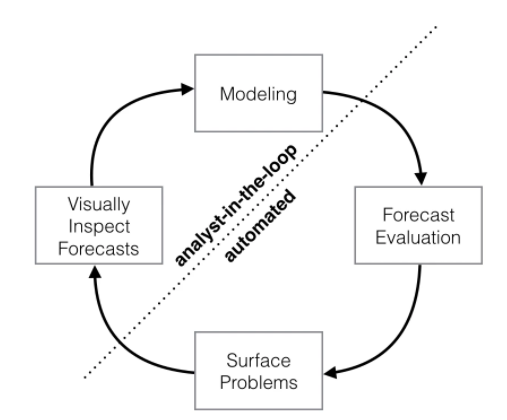
\includegraphics[width=1.00000\textwidth]{analyst in the loop.png}\\
\emph{Figure 2: Illustration of Prophets' automated forecasting
procedure with an analyst in the loop} (Taylor and Letham 2017)

The interpretability of Prophets' model parameters stems from the
mathematical formulation of the forecasting model. The formulation
posits that the series is generated by an additive, parametric function
of time \(r(t)\), defined by,
\[ r(t) = g(t) + s(t) +  h(t) + \epsilon_t.\] The additive components
include growth, seasonality and a component that adjusts for holidays as
well as once-off events e.g.~anticipated market shocks in the instance
of financial time series.

The growth component, \(g(t)\), is modelled using a generalized form of
the logistic population growth model and is of the form;\\
\[g(t) = \frac{C(t)}{1+exp(-(k+\boldsymbol{a}(t)^T \delta(t-(b+\boldsymbol{a}(t)^T \gamma)))}\]\\
Where:\\
\(\bullet C(t)\) represents the carrying capacity of the growth
component and can be modelled using a polynomial function of time, the
simplest being a constant or linear model.\\
\(\bullet (k+\boldsymbol{a}(t)^T\delta)\) is the growth rate factor with
the \(\boldsymbol{a}(t)^T\delta\) term enabling the forecaster to choose
where the growth rate changes( i.e change points) and\\
\(\bullet (b+\boldsymbol{a}(t)^T \gamma)\) is the adjusted offset
parameter.

The growth component of the model has two useful features that allow the
carrying capacity and growth rate of the model to vary with time. This
enables an analyst to manually define when and how the growth rate
changes at different change points (Taylor and Letham 2017). This
feature is particularly useful for forecasting stock price data since
analysts are able to incorporate market movements that lead to the
growth rate either decreasing, increasing or becoming constant.\\
The seasonality component, \(s(t)\) with periodicity \(P\) is given by,
\[s(t) = \sum_{n = -N}^{N}c_n \exp(j\frac{2\pi nt}{P})\]

Yearly and weekly seasonality is modelled using the standard Fourier
series. Analysts can thus use prior knowledge to account for the effects
of periodicities they have observed seasonally which is similar to the
periodicity of Seasonal ARIMA models.

Lastly, \(h(t)\) is the holiday and events component, a feature that
ARIMA models are not adapted to. The holiday component enables analysts
to incorporate shocks and once-off events that do not follow a periodic
pattern but may have an effect on the price of a stock. Holidays and
events are modelled using,

\[ h(t) = \sum_{j = 1}^{L}\kappa_j \boldsymbol{1}(t \in D_j) \label{eqn5}
\] Where, \(\kappa\) is a normally distributed scaling factor and
\(D_j\) is a set of past and future dates where holidays or events
occur.

Prophet translates model parameter estimation into a curve-fitting
exercise by employing Maximum Apriori Posterior (MAP) estimation, a
Bayesian approach to estimating optimal parameter values for the
forecasting model. MAP estimation finds the maximum posterior estimates
for the parameters by using the likelihood function and an apriori
distribution to evaluate a posterior distribution which is then
optimized to return point estimates of the parameters (Taylor and Letham
2017). Thereafter, the package automatically evaluates the forecasts by
comparing the Simulated Historical Forecast (SHF) errors of baseline
forecasting methods (including ARIMA forecasts) to those of Prophet. SHF
errors are forecast errors generated from random points in the history
of the time series model. In Prophet, SHF errors are compared visually
to allow the analysts to easily adjust the interpretable parameters
before automatically estimating the model and evaluating forecasts.

\section{Data}\label{data}

The data set used throughout this paper comprises of the daily closing
prices of the equally-weighted FTSE/JSE Top40 price index for the five
year period from 31/07/2012 to 30/07/2017. This equates to a total of
1766 trading days excluding weekends and holidays. This period was
chosen for its recency and to avoid exposing the results to the noise
associated with the high volatility experienced in the stock market
during the 2008 financial crisis. The aim is to compare the predictive
accuracy of the two models under standard market conditions before other
confounding factors can be closely analysed. Figure 3 shows the actual
realisations of the price index data which was sourced from Datastream.

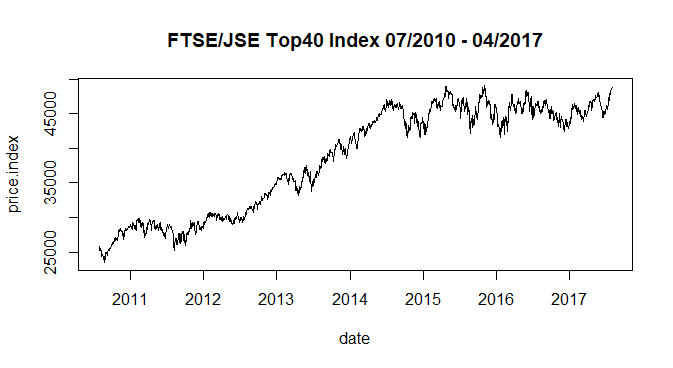
\includegraphics[width=1.00000\textwidth]{plot of Price index.png}\\
\emph{Figure 3: Realisation of the FTSE/JSE Top40 Price Index over the
period of study}

The price index was transformed to log returns as a means of avoiding
spurious regression issues which can be caused by the existence of unit
roots in stock price data.

In this paper, the \textbf{log return}(which will be used
interchangeably with \textbf{return}), over the period \([t,t+1]\) is
denoted by \(r_t\), and was calculated by evaluating;\\
\[
r_t = log(\frac{P_{t+1}}{P_t})  \label{eq1}
\]\\
Where \(P_t\) and \(P_{t+1}\) represent the price of the index at time
\(t\) and \(t+1\) respectively.

\section{Methodology}\label{methodology}

Preliminary data processing was done to clean and transform the data
before formally testing for outliers. The data was then split into
in-sample and out-of-sample periods. The in-sample period comprises of
1400 trading days from 30 July 2012 to the 1 May 2016. The out-of-sample
period comprises of the remaining 366 trading days from the dataset.

The in-sample data was used to identify the ARIMA forecasting model
using the method outlined by Box and Jenkins (1970) for building and
estimating an ARIMA model.\\
Thereafter, one-step rolling forecasts with re-estimation as outlined by
Hyndman (2014) were evaluated for an automated Prophet model and the
ARIMA model that was identified using the Box-Jenkins methodology. This
procedure was then repeated for a 5-step and 20-step forecast horizon in
order to determine whether the performance of the models vary when
estimating weekly or monthly stock returns.

The forecasts generated above where then used to calculate
\textbf{h-step rolling forecast errors} for both the ARIMA and Prophet
models. For each time point \(t\) in the out-of-sample period, the
rolling forecast error is given by,

\[ \hat{e_t} = r_t - \hat{r_t},\] where \(r_t\) is the actual return and
\(\hat{r_t}\) is the rolling forecast at time \(t\).\\
Summary statistics of the errors where used to compare the performance
of the forecasting models before a formal statistical test was done
using a Diebold-Mariano evaluation.

\section{Results}\label{results}

\subsection{Box-Jenkins Methodology: Arima Model Identification and
Selection}\label{box-jenkins-methodology-arima-model-identification-and-selection}

To identify what ARIMA model to use, the methodology as outlined in Box
and Jenkins (1970) was applied to the data. Firstly, stationarity
conditions were verified formally by performing an Augmented
Dickey-Fuller test on the in-sample returns data. The results of the
test suggest the p\_value is less that 1\%, which implies that the
in-sample returns series is stationary. The results in the
autocorrelation(ACF) and partial autocorrelation(PACF) function
illustrated in Figure 4 suggest that the second lag of both functions
might be significantly different from zero.\\
\includegraphics[width=1.00000\textwidth]{acf \& pacf plot.png}\\
\emph{Figure 4 : ACF and PACF plots for in-sample data}

Observations from the above plots informed the choice of candidate
\emph{ARIMA(p,d,q)} models to fit to the data. The candidate models that
were fit to the in-sample data are shown in Table 1 with their
respective AIC values. The candidate model with the lowest AIC is the
\(ARIMA(2,0,2)\). This model was thus selected as the ARIMA forecasting
model.\\
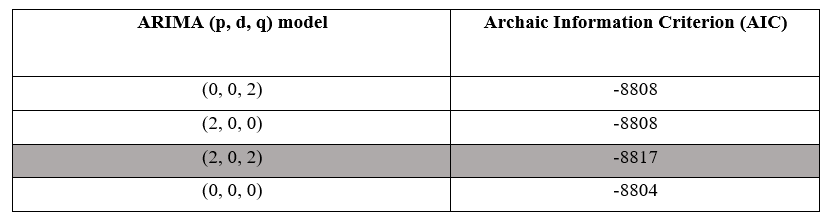
\includegraphics[width=1.00000\textwidth]{AIC.png}\\
\emph{Table 1: AIC for Candidate ARIMA models}

\subsection{Forecast Error Evaluation}\label{forecast-error-evaluation}

The results of model estimation and forecast evaluation using the
rolling window for h-step forecasts yielded forecasts errors with
roughly equal distributions. This is visible from the boxplot in Figure
5. The presence of outliers seems consistent across the different models
\textbf{and} forecasting horizons. Furthermore, variations in accuracy
across different forecasting horizons \emph{for each} model is not
observable in Figure 5. The mean error and spread of both models across
different time horizons appears to be constant.
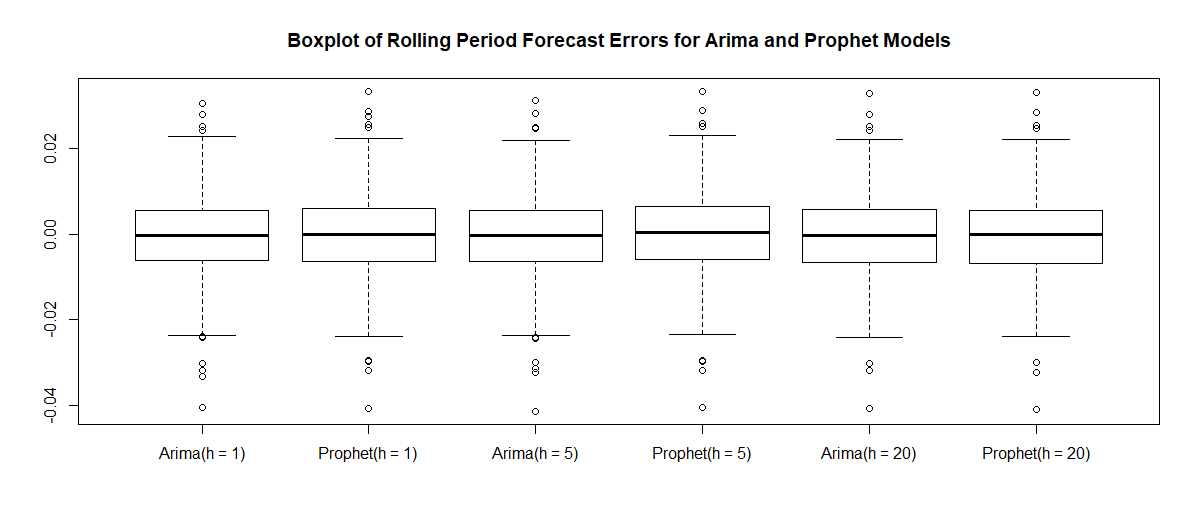
\includegraphics[width=1.05000\textwidth]{Forecast error boxplot.png}\\
\emph{Figure 5: Boxplot illustrating distribution of rolling forecast
errors for different time horizons, h}

\subsubsection{Forecast Error
Statistics}\label{forecast-error-statistics}

Table 2 summarizes the forecast error statistics for both the ARIMA and
Prophet model across the three different time horizons.\\
Across all forecast horizons, the ARIMA model appears to be
overestimating returns. This is evident from the negative mean error(ME)
across \(h = (1,5,20)\). On the contrary, the Prophet model
underestimates the forecasts for one-step and five-step ahead
forecasting horizons. It then overstimates returns when forecasting
twenty-steps ahead. The ME results shown in Table 2 fail to clearly
illustrate which model performs better. Furthermore, the ME values are
relatively small when compared against other error statistics.

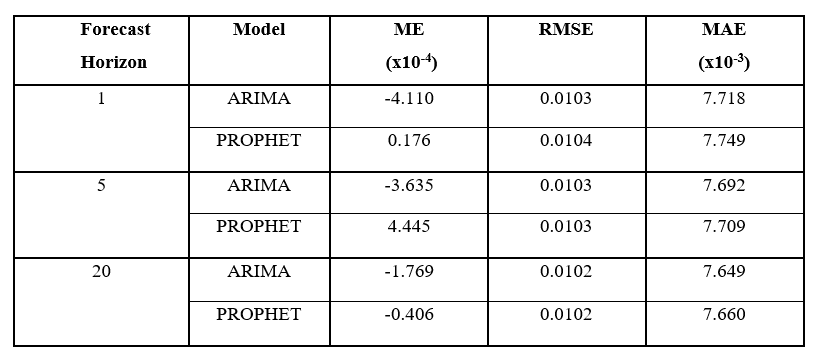
\includegraphics[width=1.00000\textwidth]{error stats.png}\\
\emph{Table 2 : Forecast error diagnostic statistics over different
forecasting horizons}

The Root Mean Square Error (RMSE) across different forecast horizons and
across both models are considerably close to each other in value
relative to the other error statistics. The same observation can be made
for the Mean Absolute Errors (MAE). These results suggest that the
models possibly have the same forecasting accuracy.

\subsubsection{Diebold-Mariano
Evaluation}\label{diebold-mariano-evaluation-1}

The observations made from Table 2 in section 5.2.1 suggest that the
ARIMA and Prophet models have equal predictive accuracy. These
assertions can be formally quantified through a Diebold-Mariano(DM) test
which evaluates whether the models have equal predictive accuracy
against the alternative hypothesis that one model has superior accuracy
over the other. Table 3 reports the results obtained when the rolling
forecast errors were formally compared against each other over different
time horizons.\\
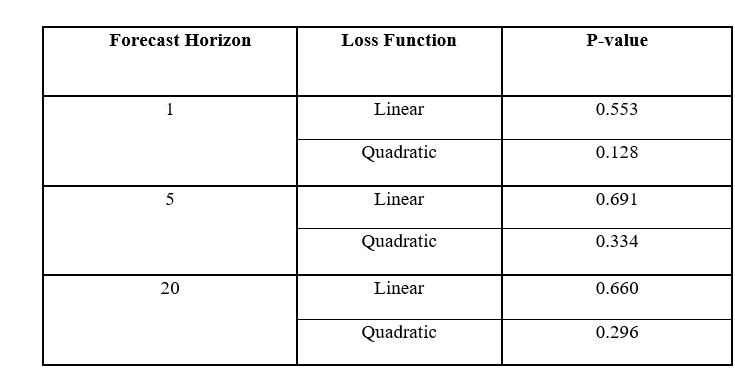
\includegraphics[width=1.05000\textwidth]{dm results.png}\\
\emph{Table 3 Results of the Diebold-Mariano Hypothesis Test}\\
The p-value across all the time horizons for either linear and quadratic
loss functions suggest that we would fail to reject the null hypothesis.
This implies that the predictive accuracy of the models could be equal.
These results formally validate the observations made obtained in
section 5.2.1.

\section{Discussion of Results}\label{discussion-of-results}

The results of the study show that there is no significant evidence to
conclude that Prophet generates superior forecasts for returns on the
FTSE/JSE Top40 Index when compared against those of an ARIMA model when
the Diebold-Mariano Test is used as a method of evaluation. These
results are consistent for daily, weekly and monthly forecasting
horizons.\\
Nevertheless, the study has flagged the possibility that, on average,
the ARIMA model tends to overestimate forecasted returns on the index
for the forecast horizons under consideration. This is contrary to
Prophet, that, on average, underestimates forecasted returns over daily
and weekly time horizons. This information could be useful for an
analyst engaged in short-term strategies since the choice of the
forecasting model can reflect a particular sentiment or risk appetite.
For example, if the analyst feels like prevailing returns are
underpriced by the market, they might choose to use an ARIMA model,
whereas an opposite sentiment could warrant the use of Prophet.\\
Furthermore, it is worth noting that the merits of Prophet may have not
been fully exposed in this study due to the use of transformed data and
the choice of a forecasting horizon that excluded periods of high
volatility. Nonetheless, it is reassuring that the model has performed
as well as the ARIMA model. This observation could create room for the
application of Prophet in circumstances where flexibility in the model
formulation is desireable.

\section{Conclusion}\label{conclusion}

The challenge of building models that generate superior stock return
forecasts has led to widespread research in the field of quantitative
analysis for decades, but the ARIMA model remains the standard against
which to compare new innovations. This is because of its relative
simplicity and ability to evolve into more complex applications e.g in
the hybrid models considered in the literature review.\\
Prophet has reduced the problem of estimating a time series model to a
curve fittig exercise by defining an additive, parametric function of
time. The functions' parameters are then estimated using Bayesian
estimation methods after which the tool automatically executes forecast
evaluation to optimize its predictive ability.\\
The results of this study suggest that, using a Diebold-Mariano
evaluation, the ARIMA and Prophet forecasting models do not have a
significant difference in predictive accuracy across time horizons of up
to a month. The implications of this are that analysts can then choose
which model to use based on their needs without significantly
compromising forecast accuracy.\\
This study was confined to the analysis of predictive performance during
general market conditions. Further research could explore the predictive
ability of the models during different market conditions. For example,
performance can be compared during bull and bear market conditions or
during periods of high volatility. Additionally, further research can
assess whether prophet would perform better on raw data that has not
been transformed, since the model is built with growth and seasonality
components. This use of which could lead to Prophet models that generate
superior forecasts when compared against alternatives.

\section*{References}\label{references}
\addcontentsline{toc}{section}{References}

\hypertarget{refs}{}
\hypertarget{ref-adebiyi2014comparison}{}
Adebiyi, Ayodele Ariyo, Aderemi Oluyinka Adewumi, and Charles Korede
Ayo. 2014. ``Comparison of Arima and Artificial Neural Networks Models
for Stock Price Prediction.'' \emph{Journal of Applied Mathematics}
2014. Hindawi Publishing Corporation.

\hypertarget{ref-box1970time}{}
Box, George Edward P, and Gwilym M Jenkins. 1970. ``Time Series
Analysis: Forecasting and Control, 1976.'' \emph{ISBN: 0-8162-1104-3}.

\hypertarget{ref-givoly1984quality}{}
Givoly, Dan, and Josef Lakonishok. 1984. ``The Quality of Analysts'
Forecasts of Earnings.'' \emph{Financial Analysts Journal}. JSTOR,
40--47.

\hypertarget{ref-guerard1989combining}{}
Guerard, John B. 1989. ``Combining Time-Series Model Forecasts and
Analysts' Forecasts for Superior Forecasts of Annual Earnings.''
\emph{Financial Analysts Journal}. JSTOR, 69--71.

\hypertarget{ref-RJHyndman2014}{}
Hyndman, Robert J. 2014. ``Variations on Rolling Forecasts.''
\url{https://robjhyndman.com/hyndsight/rolling-forecasts/}.

\hypertarget{ref-kihoro2004seasonal}{}
Kihoro, J, R Otieno, and C Wafula. 2004. ``Seasonal Time Series
Forecasting: A Comparative Study of Arima and Ann Models.'' \emph{AJST}
5 (2).

\hypertarget{ref-kriesel2007brief}{}
Kriesel, David. 2007. ``A Brief Introduction on Neural Networks.''
Citeseer.

\hypertarget{ref-lin2009short}{}
Lin, Xiaowei, Zehong Yang, and Yixu Song. 2009. ``Short-Term Stock Price
Prediction Based on Echo State Networks.'' \emph{Expert Systems with
Applications} 36 (3). Elsevier: 7313--7.

\hypertarget{ref-Mariano2000}{}
Mariano, Robert S. 2000. ``Testing Forecast Accuracy.'' University of
Pennsylvania; Course Notes.

\hypertarget{ref-moreno2011artificial}{}
Moreno, Juan José Montaño, Alfonso Palmer Pol, and Pilar Muñoz Gracia.
2011. ``Artificial Neural Networks Applied to Forecasting Time Series.''
\emph{Psicothema} 23 (2): 322--29.

\hypertarget{ref-Muten2014}{}
Mutendadzamera, S, and Farikayi K Mutasa. 2014. ``Forecasting Stock
Prices on the Zimbabwe Stock Exchange (Zse) Using Arima and Arch/Garch
Models.'' \emph{International Journal of Management Sciences} 3 (6):
419--32.

\hypertarget{ref-segaran2007programming}{}
Segaran, Toby. 2007. \emph{Programming Collective Intelligence: Building
Smart Web 2.0 Applications}. `` O'Reilly Media, Inc.''

\hypertarget{ref-tanikic2012artificial}{}
Tanikic, Dejan, and Vladimir Despotovic. 2012. ``Artificial Intelligence
Techniques for Modelling of Temperature in the Metal Cutting Process.''
In \emph{Metallurgy-Advances in Materials and Processes}. InTech.

\hypertarget{ref-taylor2017forecasting}{}
Taylor, Sean J, and Benjamin Letham. 2017. ``Forecasting at Scale.''

\hypertarget{ref-wang1996stock}{}
Wang, Jung-Hua, and Jia-Yann Leu. 1996. ``Stock Market Trend Prediction
Using Arima-Based Neural Networks.'' In \emph{Neural Networks, 1996.,
Ieee International Conference on}, 4:2160--5. IEEE.

\hypertarget{ref-zahedi2015application}{}
Zahedi, Javad, and Mohammad Mahdi Rounaghi. 2015. ``Application of
Artificial Neural Network Models and Principal Component Analysis Method
in Predicting Stock Prices on Tehran Stock Exchange.'' \emph{Physica A:
Statistical Mechanics and Its Applications} 438. Elsevier: 178--87.

\hypertarget{ref-zhang2009stock}{}
Zhang, Yudong, and Lenan Wu. 2009. ``Stock Market Prediction of S\&P 500
via Combination of Improved Bco Approach and Bp Neural Network.''
\emph{Expert Systems with Applications} 36 (5). Elsevier: 8849--54.

\newpage
\renewcommand{\baselinestretch}{1}
\nocite{*}
\bibliography{}

\end{document}
